\begin{center}
    \textbf{--------- Lezione 9 - 12 aprile 2021 ---------}
\end{center}

\section{Pre-processing}
I flussi di dati devono essere trasformati in vettori n-dimensionali in modo tale da poter usare tecniche di apprendimento supervisionato per riconoscere attività.

Il pre-processing è una fase che precede la classificazione e necessita di tuning. 
Dopo la misurazione dei dati, abbiamo le seguenti fasi, come in figura \ref{fig:pipeline}:
\begin{figure}[!ht]
    \centering
    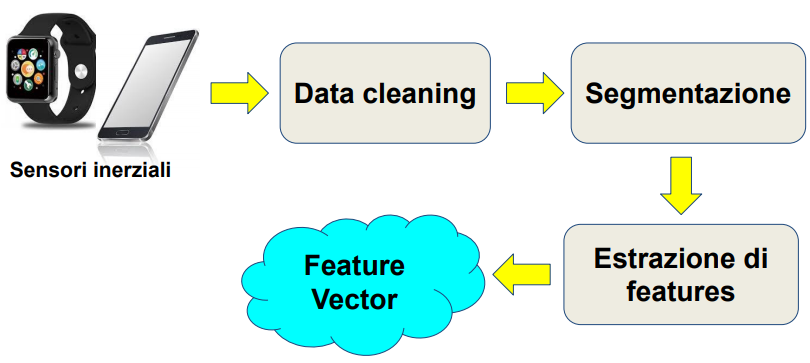
\includegraphics[width=.6\textwidth]{images/MobiDEV/6. activity recognition/pre-processing pipeline.PNG}
    \caption{Pipeline pre-processing}
    \label{fig:pipeline}
\end{figure}

\begin{itemize}
    \item data cleaning: i dati dei sensori sono affetti da rumore e per poter rimuoverlo si utilizzano i filtri, come il filtro mediano:
    \begin{center}
        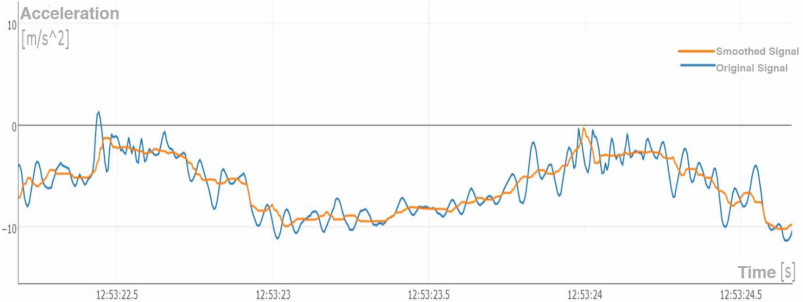
\includegraphics[width=\textwidth]{images/MobiDEV/6. activity recognition/data cleaning.PNG}
    \end{center}
    La linea arancione rappresenta il valore del filtro, quella blu rappresenta i dati grezzi. Ogni valore del segnale viene sostituito con la mediana considerando i valori nell'intorno
    \item segmentazione: il segnale viene diviso in segmenti temporali dove ogni segmento contiene i dati di tutti i sensori presi nello spazio temporale $t_1 t_2$. La tecnica più nota è lo sliding window. Abbiamo un insieme di finestre, dove una finestra può partire a metà della finestra precedente facendo un overlap (la seconda finestra può partire a metà della prima). 
    \begin{center}
        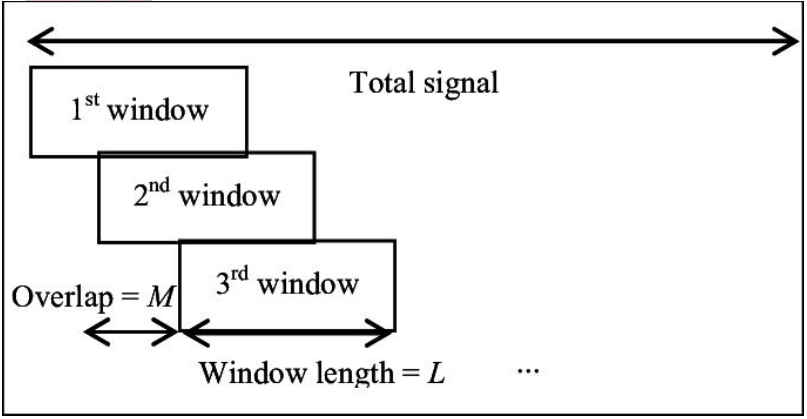
\includegraphics[width=.75\textwidth]{images/MobiDEV/6. activity recognition/segmentazione.PNG}    
    \end{center}
    Questo avviene perché andremo a classificare ognuna di queste finestre. Se le finestre sono affiancate senza overlap rischiamo che ci sia un'azione caratteristica che finisca a cavallo tra due e non riusciamo a riconoscerla. 
    \\ Se consideriamo attività semplici (camminare, stare seduti), di solito la finestra è di 3 o 4 secondi con un overlap del 50\%. Attività più complesse come lavare i piatti, richiedono una finestra più lunga. La dimensione della finestra può essere scelta anche in base a quanto "real-time" vuole essere il sistema 
    \item feature extraction: dai segmenti estraiamo informazioni per creare i vettori, i \textbf{feature vector}.
    
\end{itemize}

\subsection{Features}
Ci sono due tipi di feature, basate:
\begin{itemize}
    \item sul tempo: caratteristiche del segnale che riflettono il suo andamento nel tempo (es: media, varianza, ecc.)
    \item sulla frequenza: caratteristiche del segnale che riflettono la sua periodicità
\end{itemize}

\subsubsection{Generazione del feature vector}
Per ogni dispositivo mobile dell'utente si calcolano le features per ogni sensore inerziale al suo interno. Le features vengono concatenate per generare un vettore n-dimensionale, dove n è il numero di features calcolate. Le features sono solitamente grandi un centinaio. I range di valori delle diverse features possono variare significativamente.

\subsubsection{Feature scaling}
Per costruire un modello di riconoscimento robusto, abbiamo due tecniche:
\begin{itemize}
    \item normalizzazione: vengono normalizzati i range delle features e i valori sono scalati nel range [0,1]. È utile per rappresentare i dati usando una scala comune
    \item standardizzazione: cerca di riportare feature con range diversi, su una distribuzione simile. I valori sono centrati in 0. È particolarmente adatta se i dati hanno una distribuzione gaussiana 
\end{itemize}

Nell'ambito dell'activity recognition, non sempre normalizzare le features migliora il riconoscimento. Va valutato empiricamente se normalizzare e come. 

\section{Riconoscimento di attività: classificazione}
Abbiamo ottenuto i dati dei sensori divisi in segmenti e la notazione delle attività (etichette). La lunghezza dei segmenti dei dati non combacia con la lunghezza dei segmenti delle attività svolte. 
Serve un modo per associare un'etichetta ad ogni segmento. 
\begin{center}
    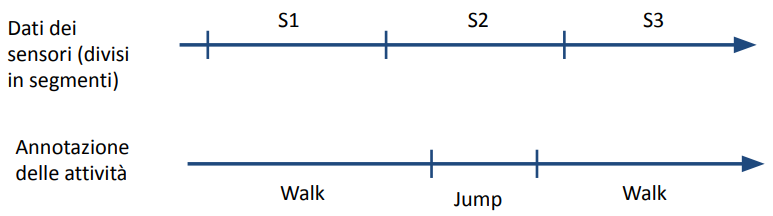
\includegraphics[width=.7\textwidth]{images/MobiDEV/6. activity recognition/labeling dei segmenti.PNG}
\end{center}

La soluzione più comune è associare l'attività prevalente del segmento. Ad esempio in S2, l'attività prevalente è Jump. In alcune situazioni, questa tecnica non funziona.

\subsection{Algoritmi di machine learning "noti" in AR}
Una volta etichettati i segmenti possiamo addestrare il classificatore. 
Tra gli algoritmi di classificazione, i più usati sono:
\begin{itemize}
    \item Support Vector Machine (SVM): supponiamo di avere 2 attività. Pallini neri attività 2, pallini bianchi attività 1. Lo scopo è di trovare un iperpiano che cerca di dividere al meglio gli esempi dell'attività 1 da quelli dell'attività 2.
    Bisogna quindi trovare la retta che distingue meglio le attività
    \begin{center}
        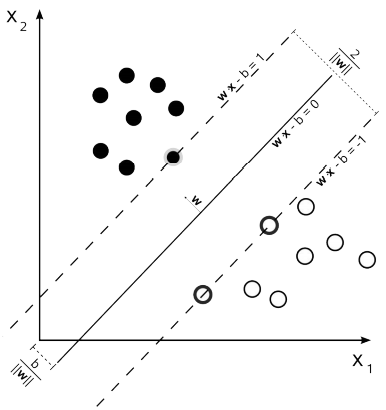
\includegraphics[width=.4\textwidth]{images/MobiDEV/6. activity recognition/svm.PNG}
    \end{center}
    \item Random Forest (basati su Decision Tree): il decision tree è un albero costruito in fase di training. Ogni nodo di questo albero è una condizione su una specifica feature (ad esempio valore dell'accelerometro $<$ 34). 
    Sono condizioni calcolate automaticamente in base ai dati di training. Le foglie di questo albero sono le attività. Si parte dalla radice e si passa attraverso l'albero in base alle condizioni che si trovano in ogni nodo.
    \begin{center}
        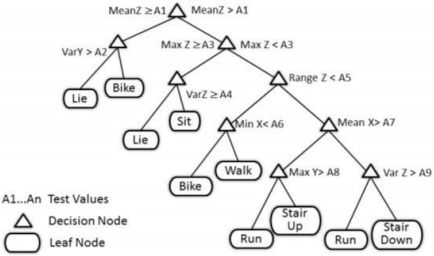
\includegraphics[width=.7\textwidth]{images/MobiDEV/6. activity recognition/decision tree.PNG}
    \end{center}
    Il random forest è una foresta di alberi di decisione. Il feature vector attraversa tutti i decision tree. Ogni albero di decisione è formato in modo randomico ed ognuno arriva alla propria predizione di attività. Attraverso un majority-voting viene presa l'attività prevalente tra tutti i decision tree. 
    \begin{center}
        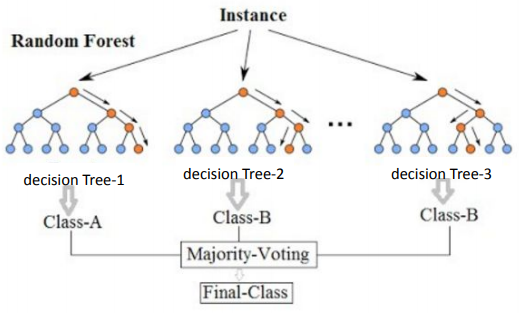
\includegraphics[width=.7\textwidth]{images/MobiDEV/6. activity recognition/random forest.PNG}
    \end{center}
    \item Reti neurali: ci sono tecniche di deep learning che permettono di calcolare le feature in modo indipendente. 
    Per estrarre le feature in modo affidabile, sono necessari molti dati
     \begin{center}
        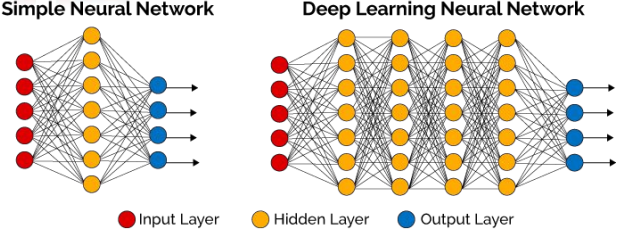
\includegraphics[width=.7\textwidth]{images/MobiDEV/6. activity recognition/reti neurali.PNG}
    \end{center}
\end{itemize} 

\subsection{Modello di riconoscimento}
Il modello di riconoscimento può essere:
\begin{itemize}
    \item personalizzato: allenato solo con dati dell'utente che utilizza il sistema. È molto accurato, ma non è realizzabile
    \item generalizzato: allenato usando dati di utenti diversi da colui che usa il sistema. Il training viene fatto una volta sola, ma il riconoscimento spesso è meno accurato. 
    Le API di Google e Apple adottano questo modello
\end{itemize}

L'ideale sarebbe avere un modello che combini i vantaggi dei due modelli: il training set viene creato inizialmente con un set di utenti diversi da colui che utilizza il sistema e poi viene chiesto all'utente di annotare una piccola porzione di dati per personalizzare il riconoscimento.

Dobbiamo capire se fare il riconoscimento:
\begin{itemize}
    \item offline: raccoglie i dati per un certo periodo e successivamente fa il riconoscimento
    \item online: processa i dati per riconoscere le attività in real-time. Lato online abbiamo pro e contro:
    
    \begin{table}[!ht]
        \centering
        \begin{tabular}{|p{.4\textwidth}|p{.4\textwidth}|}
            \hline
            \multicolumn{2}{|c|}{\textbf{Lato server}} \\
            \hline
            \textbf{pro} & \textbf{contro}\\
            \hline
            capacità computazionali elevate & grosso overhead in termini di comunicazione di rete \\
            \hline
        \end{tabular}
    \end{table}
    \begin{table}[!ht]
        \centering
        \begin{tabular}{|p{.4\textwidth}|p{.4\textwidth}|}
            \hline
            \multicolumn{2}{|c|}{\textbf{Lato mobile}} \\
            \hline
            \textbf{pro} & \textbf{contro}\\
            \hline
            miglior supporto al riconoscimento real-time & bisogna creare modelli di riconoscimento che possano girare efficientemente su dispositivi mobili \\
            \hline
        \end{tabular}
    \end{table}
\end{itemize}

Nei dispositivi mobili, il modello deve essere creato offline usando un training set (esistono svariati tool di machine learning che permettono di farlo) e ci sono apposite librerie che caricano il modello e lo usano per riconoscere in tempo reale le attività. 
Per poter creare e deployare il modello è necessario usare la stessa SDK. 
\\ Le SDK più famose sono:
\begin{itemize}
    \item Weka per Android
    \item CoreML per iOS: si può processare un modello offline ad esempio con librerie di Python, viene validato e una volta soddisfatti lo si può convertire in un formato apposito per CoreML e poi può essere deployato sull'applicazione ed utilizzato per il riconoscimento
    \item TensorFlow Lite per deep learning che può essere integrato sia in Android che in iOS
\end{itemize}

Un tool di Apple che fa parte di XCode e che permette di addestrare un classificatore senza dover scrivere codice è CreateML.

\subsection{Uso del modello}
Una volta che il modello è stato addestrato viene usato nel seguente modo:
\begin{itemize}
    \item il dispositivo acquisisce lo stream di dati dai sensori
    \item segmenta lo stream
    \item per ogni segmento estrae il feature vector
    \item il feature vector viene dato al classificatore che restituisce l'etichetta
\end{itemize}

\subsection{Il risultato del classificatore}
Il classificatore non restituisce solo l'attività ma una distribuzione di attività. 
Ad esempio abbiamo due distribuzioni di probabilità:
\begin{itemize}
    \item Caso 1: $<A, 0.5> <B, 0.4> <C, 0.1>$ 
    \item Caso 2: $<A, 0.5> <B, 0.25> <C, 0.25>$
\end{itemize}
In entrambi i casi l'etichetta più probabile è A, anche se nel primo caso il classificatore è più incerto (A con confidenza 0.5 e B di 0.4). \\
In base alla situazione si può decidere cosa fare del risultato: 
\begin{itemize}
    \item usare sempre l'etichetta con confidenza più alta
    \item definire qualche metrica per decidere quando prendere per buono il risultato del classificatore
\end{itemize}